\documentclass[10pt,twocolumn,letterpaper,a4paper]{article}
%
\usepackage{graphicx}
\usepackage[utf8]{inputenc}
\usepackage{float} % para la posición en la pagina
\usepackage[spanish]{babel}

%Modificación del formato de los captions
\usepackage[margin=10pt,labelfont=bf]{caption}

% Modificar la fuente de los titulos: 
% 14 = tamaño fuente
% 12 = espaciado entre filas de los titulos
% 0.5em = espaciado entre el número y el texto
\usepackage{titlesec}
\titleformat{\section}{\normalfont\fontsize{14}{12}\bfseries}{\thesection.}{0.5em}{}

% Modificar los margenes del documento
\usepackage[a4paper]{geometry}
\geometry{top=0.5cm, bottom=1.5cm, left=2cm, right=2cm}

% Ruta de las evidencias
\graphicspath{{./imagenes/}}

\begin{document}
%
% Cabecera
%

\title{\textbf{\LARGE{Predicción de tipos de cáncer mediante \\ Aprendizaje Automático}}\\}
\author{José Antonio García García}

\twocolumn[
  \begin{@twocolumnfalse}
    \maketitle
    \begin{center}\rule{0.9\textwidth}{0.1mm} \end{center}
    \begin{abstract}
      \normalsize Este artículo realiza un estudio sobre los resultados proporcionados por varios modelos de aprendizaje automático con el fin de determinar cual es el mejor a la hora de analizar una muestra de datos sobre secuencias ARN encontradas en pacientes con diferentes tipos de tumores: BRCA, KIRC, COAD, LUAD y PRAD.   \\ \\
      \normalsize \textbf{Keywords:} detección de cáncer \textbf{·} aprendizaje automático \textbf{·} arboles de decisión \textbf{·} Knn \textbf{·} redes neuronales \textbf{·} máquinas vector soporte
      \begin{center}\rule{0.9\textwidth}{0.1mm} \end{center}
    \end{abstract}
  \end{@twocolumnfalse}
]

%
% Texto
%

\section{INTRODUCCIÓN}

Para la realización de este estudio se ha utilizado el conjunto de datos creado por la "\textit{UCI Machine Learning Repository"} en base a una muestra aleatoria del conjunto de datos recabados por "\textit{The Cancer Genome Atlas Pan-Cancer analysis project}" de pacientes con diferentes tipos de tumores. El conjunto de datos inicial consta de más de 20.000 variables y 800 instancias por lo que, debido a limitaciones físicas, el estudio se ha realizado con una muestra de este conjunto.


\section{DECISIONES}

Tras escoger una muestra inicial de 100 variables y 800 instancias se creyó conveniente utilizar un esquema de validación cruzada con un valor k por defecto de 10, ya que el gran número de variables e instancias hace que un solo dato, por si mismo, no alteré en gran medida los resultados obtenidos. 
Con la muestra ya seleccionada se procedió a dividir en dos subconjuntos: entrenamiento y pruebas. Se buscó un equilibrio entre alimentar al entrenamiento con la mayor cantidad de datos posible para mejorar las predicciones y dejar una muestra representativa para las pruebas por lo que se ha asignando al conjunto de datos de entrenamiento el 75\% de las instancias y el 25\% restante para pruebas.
Tras la elección de un esquema de evaluación y la separación de la muestra en entrenamiento y pruebas se tomó la decisión de que modelos y parámetros se iban a utilizar en el estudio y los escogidos fueron:
\begin{enumerate}
  \item Arboles de decisión: se utilizaron los paradigmas C4.5 con los parámetros por defecto, RPart con 15 valores diferentes de ganancia mínima y RPart2 con una lista de 7 máximos de profundidad, el máximo disponible para esta muestra.
  \item Knn: para este paradigma se probó una lista de 100 valores distintos de k, pero se decidió utilizar una lista de 15 debido a que el valor anterior no aportaba mejoras significativas y llegaba a empeorar a partir de un k superior a 65.
  \item Redes Neuronales: para este artículo se han utilizado redes neuronales de 1, 2 y 3 capas ocultas. Se ha realizado una prueba para ver el número optimo de neuronas por capa y, tras un estudio en una red neuronal de 1 capa de entre 5 y 80 neuronas con una tasa de aprendizaje de 0.03, se ha decidido tener en cuenta los resultados obtenidos por redes que contengan entre 17 y 21 neuronas por capa, para no alargar demasiado el calculo de resultados.
  \item Maquinas Vector Soporte: en este punto se optó por probar paradigmas lineales con margen duro y con margen blando, así como polinomiales y radiales. Para el caso de los paradigmas lineales se utilizo un c de 500, mientras que para el margen blando se utilizó un c de 1. Por otro lado, para analizar los resultados de los paradigmas no lineales se decidió tomar un rango de parámetros, siendo en el caso del polinomial grados de 2 a 5, al igual que para c y una escala de 0.1, 0.5 y 1; y en el caso del radial con un valor de sigma de entre 3 y 7 y un valor de c de 1, 5 y 10.
\end{enumerate}

\section{ANÁLISIS DE RESULTADOS}

Tras entrenar los anteriores paradigmas con el conjunto de datos la grafica que se muestra a la hora de realizar las pruebas es la que aparece en la \textbf{Figura \ref{figura_1}}.

\begin{figure}[!htbp] 
  \centering 
  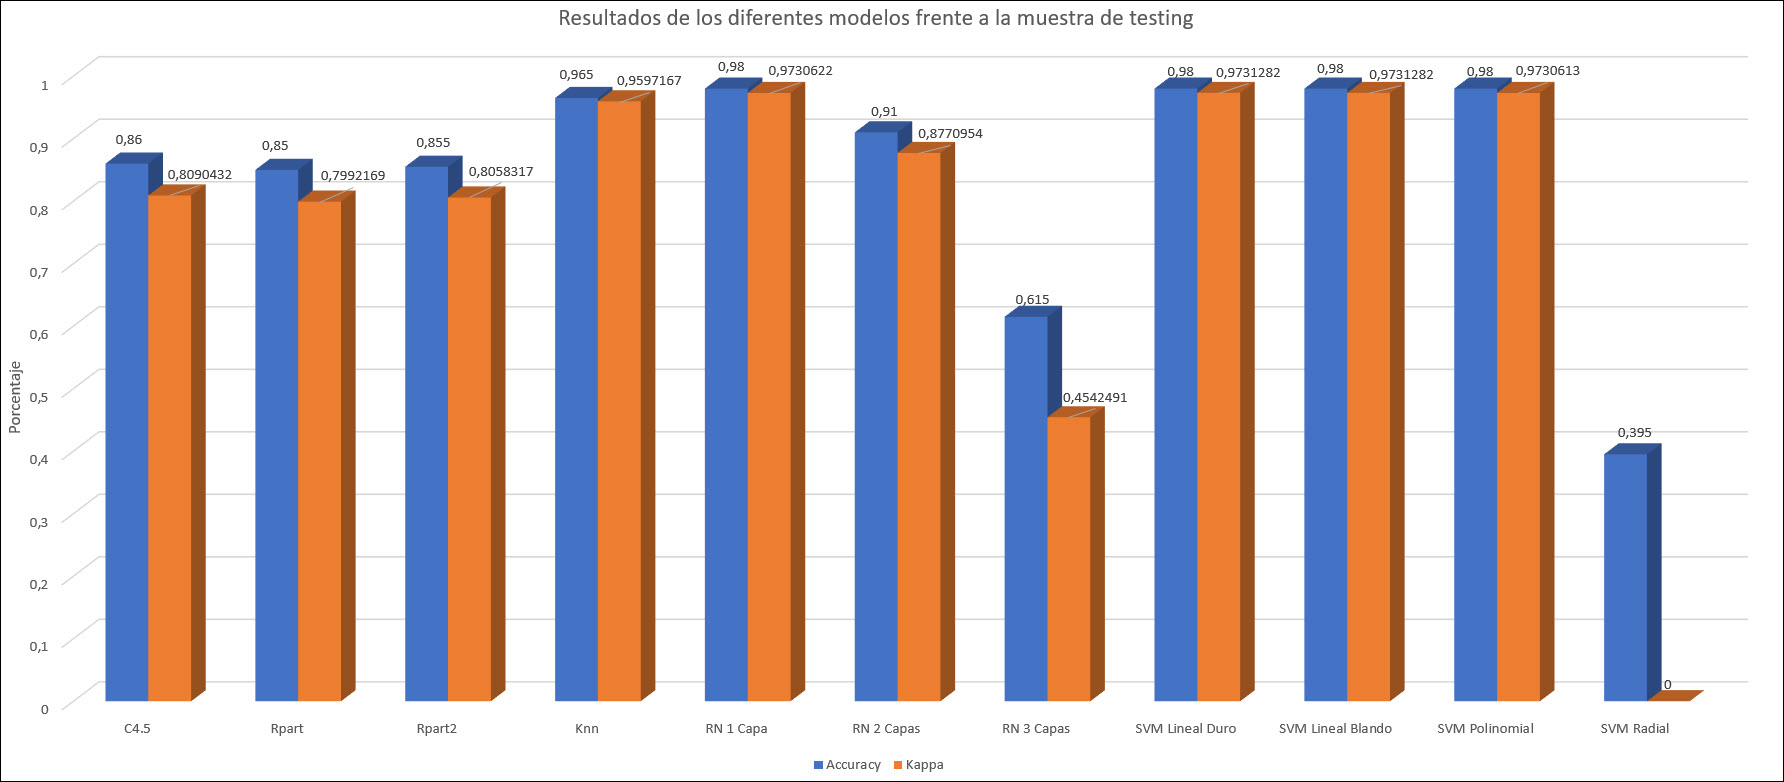
\includegraphics[width=8cm]{Resultados.jpg}\\ 
  \caption{Resultados de los diferentes modelos.}
  \label{figura_1} 
\end{figure} 

Antes de pasar a analizar los resultados es necesario escoger que parámetro se utilizará para compararlos y, en este estudio, debido a la predominancia de la secuencia genética BRCA frente al resto, apareciendo en más del doble de ocasiones que la segunda secuencia genética más común, se ha tomado la decisión de utilizar el valor Kappa para evitar cualquier desbalance en los resultados.

Para entrar más en detalle los paradigmas se separarán en dos grupos: los que tienen un porcentaje de Kappa inferior a 0.95 y los que están por encima de ese valor.

Dentro del primer grupo se encuentran los arboles de decisión, las redes neuronales de más de una capa y la SVM radial. Este subgrupo también seria susceptible a ser dividido en dos ya que los resultados obtenidos de los arboles de decisión y de la red de dos capas son bastante buenos, entre el 0.80 y el 0.85, y distan mucho de los pésimos valores ofrecidos por la red neuronal de 3 capas, 0.45, y de la SVM, 0. Estos dos últimos los desecharemos desde el primer momento. En el caso del paradigma C4.5 no se observa una gran variabilidad en los datos si cambiamos los parámetros, por lo general son bastante buenos, lo cual no ocurre con RPart y RPart2 que tienden a sobreajustar mucho los resultados y cuando se utilizan parámetros más reales cae bastante su exactitud. En el caso de la red neuronal de 2 capas vemos como a medida que aumenta el número de neuronas van mejorando sus resultados, pero siguen estando lejos tanto en exactitud como en tiempo si los comparamos con la red de 1 capa.

Si pasamos al segundo subgrupo nos encontramos con resultados muy interesantes, rodando un Kappa de 0.973  en el caso de la red neuronal de 1 capa, y las SVM lineales y polinomial, un poco menos exacto es el Knn con un Kappa de 0.959. Con estos valores de Knn podemos asegurar que no hay variables inservibles, ya que sino Knn saldría perjudicado. Estudiando los resultados de la red neuronal podemos ver como tiende a mejorar a mayor cantidad de neuronas por capa, pero también aumenta el tiempo empleado en calcularlo. Por último, las maquinas de vector soporte han dado muy buenos resultados tanto en el conjunto de datos de entrenamiento como en el de prueba; también podemos asegurar que las regiones de los datos están bien alejadas unas de otras ya que el rendimiento ofrecido por el margen duro y el margen blando no ha influido en los resultados.

\section{Conclusión}

Por ultimo voy a tratar de explicar porque he escogido el paradigma Knn como el mejor para este problema y como he llegado a esta conclusión. 

Para empezar es necesario decir que todos los paradigmas que entraban en el subgrupo de un Kappa inferior a 0.95 también cumple que, si comparamos sus resultados mediante binom-test frente a los resultados del Knn, nos sale siempre un valor inferior al 0.05, por lo que se puede asegurar que Knn es mejor. También se han comparado su desempeño en el entrenamiento mediante t-test frente al Knn y se puede asegurar que Knn es mejor que todos ellos.

Sin embargo estás decisiones no pueden ser aplicadas al grupo que obtuvo unos resultados de Kappa superiores a 0.95, ya que de entre ellos ninguno puede asegurarse que es mejor que los demás mediante estos test; de hecho los resultados mostrados por Knn son ligeramente peores. Tampoco se puede argumentar que los valores varían mucho entre entrenamiento y pruebas, ya que están bastante parejos. Por estás razones cualquiera de los paradigmas de este subgrupo serian totalmente validos.

Como ultimo pilar para apoyar la elección de Knn, se ha utilizado el tiempo empleado en entrenar el paradigma. Si se observa la \textbf{Figura \ref{figura_2}} se puede observar que solo aparecen 4 paradigmas y esto es porque la red neuronal ha sido descartada desde un principio ya que desvirtuá el resto de resultados, por lo que no se puede comparar en cuanto al tiempo empleado con los demás. De los 4 restantes, el polonomial es el peor, seguido de las dos versiones del lineal y el mejor es el Knn con un tiempo estimado de 0 segundos. Esto quiere decir que, con la muestra aplicada al estudio, el tiempo empleado por el Knn es despreciable. Todos los tiempos aumentarán a medida que crezca el número de variables, he incluso Knn llegará a necesitar cierto tiempo de computación, pero este valor será muy inferior a los demás si tenemos en cuenta el conjunto de datos inicial, de 20.000 variables, donde el Knn sería el más optimo en cuanto a resultados frente a tiempo.

\begin{figure}[!htbp] 
  \centering 
  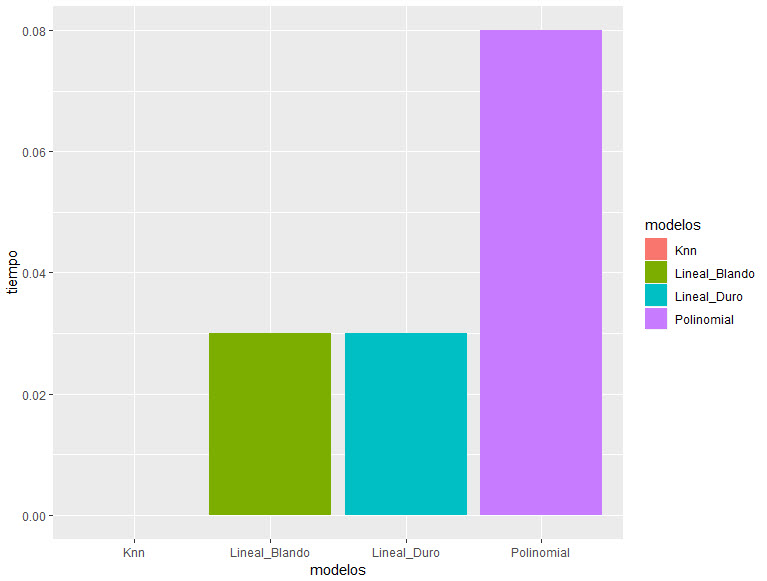
\includegraphics[width=8cm]{Tiempos.jpg}\\ 
  \caption{Tiempos empleados en el entrenamiento de los mejores modelos.}
  \label{figura_2} 
\end{figure} 

\end{document}